
\begin{asm}
  \label{asm:surfaceForceViscous}
  From now on,
  assume that
  \begin{equation}
    \label{eq:surfaceForceSigma}
    \text{force on $S$ per unit area} = -p(\mathbf{x},t)\mathbf{n}+\mathbf{n}\cdot\boldsymbol\sigma(\mathbf{x},t),
  \end{equation}
  where $\boldsymbol\sigma$ is the \emph{(deviatoric) stress tensor} and
  $\mathbf{n}$ is the unit outward normal of $S$.
\end{asm}

%%% Local Variables:
%%% mode: latex
%%% TeX-master: "../notesOnFluidMechanics"
%%% End:

\section{Spike-Train Statistics}
\label{sec:1.4}


\begin{defn}
    A complete description of the stochastic relationship between a stimulus and a response would require us to know the probabilities corresponding to every sequence of spikes that can be evoked by the stimulus.    
\end{defn}

\begin{defn}    
    Throughout this book,we use the notation P[] to denote probabilities and p[] to denote probability densities.
\end{defn}    

\begin{thm}
    The probability of a spike sequence appearing is proportional to the probability density of spike times,$p[t_1,t_2,...,t_n]$.In other words,the probability $P[t_1,t_2,...,t_n]$that a sequence of n spikes occurs with spikes ocurs with spike i falling between times $t_i$and $t_i+\vartriangle t$ for i = 1,2,...,n is given in terms of this density by the relation 
    \begin{equation}
        P[t_1,t_2,...,t_n]=p[t_1,t_,...,t_n](\vartriangle t)^n.        
    \end{equation}
    \begin{proof}
    \end{proof}
\end{thm}

\begin{defn}
    A stochastic process that generates a sequence of events ,such as action potentials ,is called a pont process.    
\end{defn}

\begin{defn}
    In general, the probability of an event occurring at any given time could depend on the entire history of preceding events. 
\end{defn}

\begin{defn}
    If this dependence extends only to the immediately preceding event,so that the intervals between successive events are independent,the point process is called a renewal process.
\end{defn}


\begin{defn}
    To make the presentation easier to follow,we separate two cases,the homogeneous Poisson process,for which the firing rate is constant over time, and the inhomogeneous Poisson process,which involves a time-dependent firing rate.
\end{defn}

\subsection{The Homogeneous Poisson Process}

\begin{defn}
    We denote the firing rate for a homogeneous Poisson process by $r(t)=r$,because it is independent of time.
\end{defn}

\begin{defn}
    $P_T[n]$,which is the probality that an arbitrary sequence of exactly n spikes occurs within a trial of duration T.    
\end{defn}

\begin{thm}
    \begin{equation}
        P_T[n]=\frac{(rn)^n}{n}exp(-rT).
    \end{equation}
    This is called the Poisson distribution.
    \begin{proof}
    \end{proof}
\end{thm}

\begin{exm}
    The probabilities $P_T[n]$,for a few n values, are plotted as a function of rT in  firgue \ref{Figure 1.11 (A)} .Note that as n increase, the probability reaches its maximum at larger T values and that large n values are more likely than small ones for large T.
\end{exm}    
\begin{center}
    \label{Figure 1.11 (A)}    
    % \includegraphics[scale = 0.15]{../../../png/n_value.png}    \\
\end{center}

\begin{exm}
    Figure B shows the probabilities of various numbers of spikes occurring when the average number of spikes is 10.
\end{exm}    
\begin{center}
    \label{Figure 1.11 (A)}    
    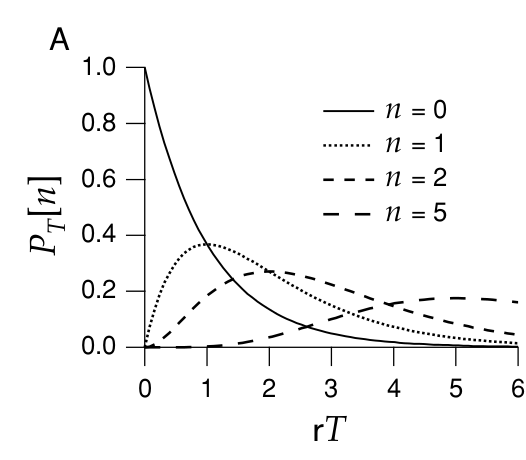
\includegraphics[scale = 0.15]{png/Figure1-4-1-A.png}\\
\end{center}



\begin{thm}
    The probability $P[t_1,t_2,...,t_n]$can be expressed in terms of another probability function $P_T[n]$,which is the probality that an arbitrary sequence of exactly n spikes occurs within a trial of duration T.Assuming that the spike times are ordered so that $0\leq t_1\leq t_2\leq ...\leq t_n\leq T$,the relationship is 
    \begin{equation}
        P[t_1,t_2,...,t_n]=n!{_T[n](\frac{\vartriangle t}{T})^n}
    \end{equation}
    \begin{proof}
    \end{proof}
\end{thm}


